%=============================================================================
%  PROGRESS REPORT (80% COMPLETION)
%  From Prediction to Action: An Explainable Web System for
%  Early Diabetes Risk Screening
%
%  COMPILE:  pdflatex progress_report.tex   (run twice, for the ToC)
%  Works on Overleaf with no extra setup.
%=============================================================================

\documentclass[11pt,a4paper]{article}

%------------------------- FILL THESE IN -------------------------------------
\newcommand{\ProjectTitle}{From Prediction to Action: An Explainable Web System
for Early Diabetes Risk Screening}
\newcommand{\SupervisorName}{[SUPERVISOR NAME]}
\newcommand{\SupervisorTitle}{[Designation, e.g.\ Assistant Professor]}
\newcommand{\StudentOne}{[STUDENT 1 NAME]}
\newcommand{\StudentOneID}{[ID]}
\newcommand{\StudentTwo}{[STUDENT 2 NAME]}
\newcommand{\StudentTwoID}{[ID]}
\newcommand{\StudentThree}{[STUDENT 3 NAME]}
\newcommand{\StudentThreeID}{[ID]}
\newcommand{\DeptName}{Department of Computer Science and Engineering}
\newcommand{\UnivName}{Islamic University of Technology}
\newcommand{\UnivCity}{Gazipur, Dhaka, Bangladesh}
\newcommand{\ReportDate}{August 2026}
%-----------------------------------------------------------------------------

\usepackage[margin=1in]{geometry}
\usepackage[T1]{fontenc}
\usepackage[utf8]{inputenc}
\usepackage{graphicx}
\usepackage{xcolor}
\usepackage{booktabs}
\usepackage{array}
\usepackage{enumitem}
\usepackage{caption}
\usepackage{fancyhdr}
\usepackage{titlesec}
\usepackage{tikz}
\usepackage{pgfplots}
\pgfplotsset{compat=1.18}
\usetikzlibrary{arrows.meta,positioning,shapes.geometric,calc,fit,backgrounds}
\usepackage[hidelinks]{hyperref}

% ---- colours ----
\definecolor{accent}{HTML}{1F6FB2}
\definecolor{soft}{HTML}{E8F1F8}
\definecolor{ok}{HTML}{0CA30C}
\definecolor{warn}{HTML}{D97706}
\definecolor{bad}{HTML}{D03B3B}
\definecolor{grayline}{HTML}{9AA5B1}

% ---- spacing / layout ----
\setlist{nosep,leftmargin=1.4em}
\titlespacing*{\section}{0pt}{1.6ex plus .3ex}{0.9ex}
\titlespacing*{\subsection}{0pt}{1.2ex plus .2ex}{0.6ex}
\titleformat{\section}{\normalfont\large\bfseries\color{accent}}{\thesection}{0.7em}{}
\titleformat{\subsection}{\normalfont\normalsize\bfseries}{\thesubsection}{0.7em}{}
\captionsetup{font=small,labelfont={bf,color=accent},skip=4pt}
% ---- LENGTH CONTROL -------------------------------------------------------
% Target is 15 pages. If the compiled PDF runs over, reduce \parskip to 0.25em
% (or 0.15em) below -- that is the single most effective lever. If it runs
% SHORT, raise it to 0.6em. Nothing else needs to change.
\setlength{\parskip}{0.38em}
% ---------------------------------------------------------------------------
\setlength{\parindent}{0pt}
\renewcommand{\arraystretch}{1.15}

\pagestyle{fancy}\fancyhf{}
\fancyhead[L]{\small\itshape From Prediction to Action}
\fancyhead[R]{\small Progress Report --- 80\%}
\fancyfoot[C]{\small\thepage}
\renewcommand{\headrulewidth}{0.4pt}

\begin{document}

%=============================================================================
% COVER PAGE
%=============================================================================
\begin{titlepage}
\centering
\thispagestyle{empty}

\vspace*{0.4cm}
{\large\scshape \UnivName\par}
{\normalsize \DeptName\par}
{\small \UnivCity\par}

\vspace{0.8cm}

\begin{tikzpicture}
  \draw[accent,line width=1pt] (0,0) -- (13,0);
\end{tikzpicture}

\vspace{1.0cm}
{\small\bfseries\color{accent} UNDERGRADUATE THESIS --- PROGRESS REPORT\par}
\vspace{0.25cm}
{\small (80\% Completion Review)\par}

\vspace{1.0cm}
{\LARGE\bfseries \ProjectTitle \par}

\vspace{0.9cm}
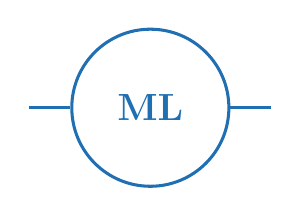
\begin{tikzpicture}[scale=0.95,transform shape]
  % small logo-ish emblem: stethoscope-free abstract mark
  \node[circle,draw=accent,line width=1.1pt,minimum size=2.1cm] (c) {};
  \node at (c) {\color{accent}\Large\bfseries ML};
  \draw[accent,line width=1.1pt] (c.east) -- ++(0.55,0);
  \draw[accent,line width=1.1pt] (c.west) -- ++(-0.55,0);
\end{tikzpicture}

\vspace{0.9cm}
{\large\bfseries Submitted by\par}
\vspace{0.35cm}
{\normalsize
\begin{tabular}{ll}
\StudentOne   & \StudentOneID \\
\StudentTwo   & \StudentTwoID \\
\StudentThree & \StudentThreeID \\
\end{tabular}\par}

\vspace{0.9cm}
{\large\bfseries Supervised by\par}
\vspace{0.3cm}
{\normalsize \SupervisorName\par}
{\small \SupervisorTitle\par}
{\small \DeptName, \UnivName\par}

\vfill

\begin{tikzpicture}
  \draw[accent,line width=1pt] (0,0) -- (13,0);
\end{tikzpicture}
\vspace{0.3cm}
{\normalsize \ReportDate\par}

\end{titlepage}

%=============================================================================
% ABSTRACT + CONTENTS  (page 2)
%=============================================================================
\setcounter{page}{2}

\section*{\color{accent}Abstract}
Type~2 diabetes is largely preventable, yet it is frequently detected only after
irreversible damage has occurred. Machine-learning risk calculators are widely
published, but most stop at producing a score: they do not tell the user
\emph{why} that score was assigned, nor \emph{what they could change}. This
project addresses that gap with a deployed, end-to-end web system that moves
from prediction to action. A gradient-boosted classifier estimates early-stage
diabetes risk on a three-level scale (Low / Medium / High); a SHAP explanation
layer attributes each individual prediction back to the factors that produced
it; and an interactive counterfactual simulator lets the user modify the
factors within their control and observe the resulting change in risk in real
time. The system is implemented as a FastAPI service and a React single-page
application, and is fully operational. This report documents the design,
implementation, and verification of the system at approximately \textbf{80\%
completion}, and sets out the remaining work: independent validation of the
model against a real-world clinical dataset, an automated test suite, and
deployment configuration.

\vspace{0.5em}
\noindent\textbf{Keywords:} explainable AI, SHAP, counterfactual explanation,
diabetes risk screening, gradient boosting, health informatics.

\vspace{0.8em}
{\color{accent}\hrule height 0.6pt}
\vspace{0.5em}

\renewcommand{\contentsname}{\color{accent}Table of Contents}
{\small\tableofcontents}

\newpage

%=============================================================================
\section{Introduction}

\subsection{Motivation}
The International Diabetes Federation estimates that 537 million adults were
living with diabetes in 2021, and that roughly one in two remained
undiagnosed~\cite{idf2021}. The clinical significance of this gap is that
Type~2 diabetes develops gradually and silently: by the time symptoms prompt a
clinical visit, vascular, renal, and retinal damage is often already
established. Crucially, the condition is also one of the most preventable
chronic diseases. The Diabetes Prevention Program trial demonstrated that a
structured lifestyle intervention reduced progression from prediabetes to
diabetes by 58\%~\cite{dpp2002}, outperforming pharmacological intervention.

The practical obstacle is not that effective interventions are unknown; it is
that individuals at risk are not identified early enough, and that those who
are identified are rarely given a concrete, personalised sense of which of
their own behaviours matter most.

\subsection{Problem Statement}
A large body of work applies machine learning to diabetes risk prediction, and
reported accuracies are frequently high. However, three limitations recur:

\begin{enumerate}[label=(\roman*)]
  \item \textbf{Opacity.} High-performing models --- gradient-boosted ensembles
        in particular --- are not directly interpretable. A user is told they
        are at ``high risk'' with no indication of why.
  \item \textbf{Non-actionability.} A risk score is a static verdict. It does
        not distinguish factors the user can change (weight, activity, diet,
        smoking) from those they cannot (age, sex, family history), and it
        offers no estimate of the benefit of changing them.
  \item \textbf{Non-deployment.} The majority of published models exist only as
        notebooks. They are never made available to the population they
        describe.
\end{enumerate}

\subsection{Contributions}
This project delivers a working system that addresses all three. Its
contributions are:

\begin{enumerate}[label=\textbf{C\arabic*.}]
  \item A three-class early-stage diabetes risk classifier deployed behind a
        documented REST API, with the training-time feature engineering
        reproduced exactly at inference time to eliminate train--serve skew.
  \item A per-prediction explanation layer using SHAP, which attributes an
        individual verdict back to the original, human-meaningful input
        features and presents them as a signed, diverging visualisation.
  \item An interactive \emph{what-if} counterfactual simulator, exposing only
        the modifiable risk factors and re-evaluating the model live as the
        user adjusts them --- converting a static score into an exploratory
        tool.
  \item A rule-based, transparent recommendation engine whose output is ordered
        by each factor's measured SHAP contribution for that specific user.
  \item An integrated educational knowledge base, so that a user receiving an
        elevated result is immediately given context rather than only a number.
\end{enumerate}

%=============================================================================
\section{Objectives and Scope}

\subsection{Objectives}
\begin{enumerate}[label=\textbf{O\arabic*.}]
  \item Train a multi-class classifier that separates Low, Medium, and High
        early-stage diabetes risk from ten routinely self-reportable inputs,
        requiring no laboratory test.
  \item Serve the model through a validated, low-latency web API.
  \item Generate a faithful per-user explanation of every prediction.
  \item Provide an interactive means of exploring how modifiable factors alter
        the predicted risk.
  \item Deliver the whole system as a usable, accessible web application rather
        than a notebook.
\end{enumerate}

\subsection{Scope and Deliberate Exclusions}
The system is a \textbf{screening and educational tool, not a diagnostic
instrument}, and this constraint shaped the design throughout. Specifically,
the following are out of scope:

\begin{itemize}
  \item \textbf{No laboratory inputs.} Fasting glucose and HbA1c are excluded
        by design. Including them would produce a far more accurate model but
        would defeat the purpose: the tool targets users who have \emph{not}
        yet been tested.
  \item \textbf{No diagnosis.} The system never asserts that a user has
        diabetes. Disclaimers appear on the result screen and in the footer of
        every page.
  \item \textbf{No data retention.} No answer is written to disk or to a
        database. Each request is stateless and independent.
  \item \textbf{No user accounts.} There is no authentication, no history, and
        therefore no personally identifiable information at rest.
\end{itemize}

%=============================================================================
\section{Background and Related Work}

\textbf{Risk scoring.} Established questionnaire instruments such as FINDRISC
and the ADA risk test use fixed additive point systems. They are transparent
and clinically validated, but their weights are static and cannot adapt to
interactions between factors.

\textbf{Machine learning approaches.} Tree ensembles consistently outperform
linear models on tabular clinical data. Gradient boosting, and XGBoost in
particular~\cite{xgboost}, has become the standard choice. Islam et
al.~\cite{islam2020} applied data-mining techniques to early-stage diabetes
symptom data, producing the widely used UCI Early Stage Diabetes Risk
Prediction dataset.

\textbf{Class imbalance and explainability.} Clinical datasets are typically
skewed toward the negative class; SMOTE~\cite{smote} synthesises minority-class
examples and is the standard remedy, provided it is applied inside the
cross-validation loop to avoid optimistic bias. For interpretation,
SHAP~\cite{shap} provides additive feature attributions with desirable
theoretical guarantees, and TreeSHAP~\cite{treeshap} computes them exactly and
efficiently for tree ensembles.

\textbf{The gap this project targets.} The literature treats explanation
largely as a tool for the \emph{model developer} --- a diagnostic aid during
training. Comparatively little work delivers explanation to the \emph{end user}
as a first-class product feature, and less still couples it with interactive
counterfactual exploration. That coupling is the distinguishing feature of this
work.

%=============================================================================
\section{System Architecture}

The system follows a three-tier separation: a presentation tier in the browser,
a stateless inference service, and the serialised model artefacts. Figure~1
shows the overall structure and the data path of a single prediction.

\begin{figure}[h!]
\centering
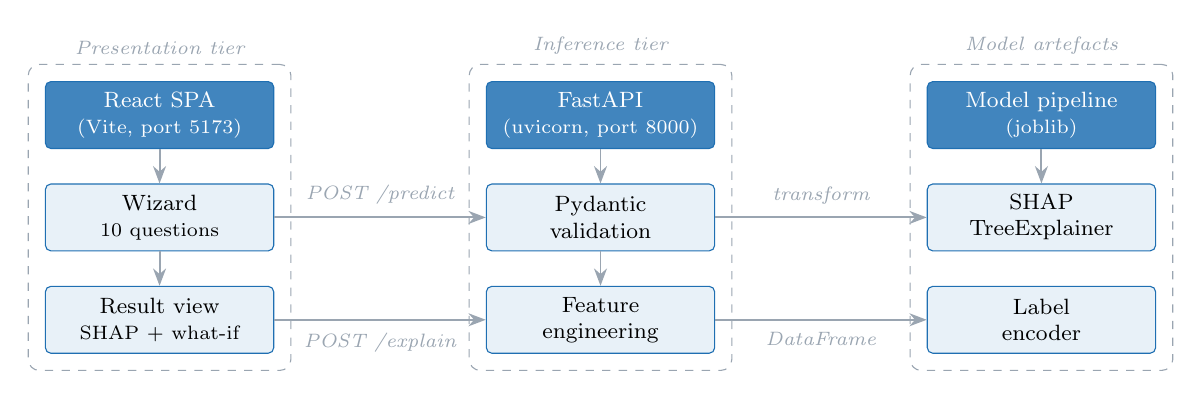
\begin{tikzpicture}[
  font=\footnotesize,
  box/.style={rectangle,rounded corners=2pt,draw=accent,fill=soft,
              minimum width=2.9cm,minimum height=0.85cm,align=center},
  dark/.style={rectangle,rounded corners=2pt,draw=accent,fill=accent!85,
              text=white,minimum width=2.9cm,minimum height=0.85cm,align=center},
  arr/.style={-{Stealth[length=2.2mm]},draw=grayline,line width=0.7pt},
  lbl/.style={font=\scriptsize\itshape,text=grayline}
]

% --- tier 1
\node[dark] (ui)   at (0,4.2) {React SPA\\\scriptsize (Vite, port 5173)};
\node[box]  (wiz)  at (0,2.9) {Wizard\\\scriptsize 10 questions};
\node[box]  (viz)  at (0,1.6) {Result view\\\scriptsize SHAP + what-if};

% --- tier 2
\node[dark] (api)  at (5.6,4.2) {FastAPI\\\scriptsize (uvicorn, port 8000)};
\node[box]  (val)  at (5.6,2.9) {Pydantic\\validation};
\node[box]  (fe)   at (5.6,1.6) {Feature\\engineering};

% --- tier 3
\node[dark] (pipe) at (11.2,4.2) {Model pipeline\\\scriptsize (joblib)};
\node[box]  (shap) at (11.2,2.9) {SHAP\\TreeExplainer};
\node[box]  (enc)  at (11.2,1.6) {Label\\encoder};

\draw[arr] (ui) -- (wiz);
\draw[arr] (wiz) -- (viz);
\draw[arr] (api) -- (val);
\draw[arr] (val) -- (fe);
\draw[arr] (pipe) -- (shap);

\draw[arr] (wiz.east) -- node[lbl,above,yshift=1pt]{POST /predict} (val.west);
\draw[arr] (viz.east) -- node[lbl,below,yshift=-1pt]{POST /explain} (fe.west);
\draw[arr] (fe.east)  -- node[lbl,below,yshift=-1pt]{DataFrame} (enc.west);
\draw[arr] (val.east) -- node[lbl,above,yshift=1pt]{transform} (shap.west);

\begin{scope}[on background layer]
  \node[draw=grayline,dashed,rounded corners,fit=(ui)(viz),
        inner sep=6pt,label={[lbl]above:Presentation tier}] {};
  \node[draw=grayline,dashed,rounded corners,fit=(api)(fe),
        inner sep=6pt,label={[lbl]above:Inference tier}] {};
  \node[draw=grayline,dashed,rounded corners,fit=(pipe)(enc),
        inner sep=6pt,label={[lbl]above:Model artefacts}] {};
\end{scope}
\end{tikzpicture}
\caption{Three-tier system architecture. The inference tier is fully stateless;
no user input is persisted at any layer.}
\end{figure}

\subsection{Design Decisions}
\begin{itemize}
  \item \textbf{Artefacts loaded once at start-up.} The pipeline, label encoder,
        SHAP explainer, and global importance table are all constructed at
        import time rather than per request. This is the principal reason the
        measured inference latency is single-digit milliseconds
        (Section~\ref{sec:results}).
  \item \textbf{Statelessness.} Because nothing is stored, the privacy claim
        made to the user is structurally guaranteed rather than merely
        promised.
  \item \textbf{Strict input contracts.} Every categorical field is typed as an
        enumeration matching the exact training vocabulary, and numeric fields
        are range-bounded. Malformed input is rejected at the API boundary and
        can never reach the model.
\end{itemize}

%=============================================================================
\section{Methodology}

\subsection{Input Features}
The model consumes ten user-supplied inputs, chosen so that every one can be
answered without a clinical test. Three engineered features are then derived
from them, giving thirteen features in total (Table~1).

\begin{table}[h!]
\centering\small
\begin{tabular}{@{}llp{6.6cm}@{}}
\toprule
\textbf{Feature} & \textbf{Type} & \textbf{Values / derivation} \\
\midrule
\multicolumn{3}{@{}l@{}}{\textit{User-supplied}}\\
gender             & categorical & Male, Female \\
age                & numeric     & 1--120 years \\
bmi                & numeric     & 10--70 kg/m$^2$ \\
physical\_activity & categorical & Low, Moderate, High \\
smoking\_habit     & categorical & Never, Former, Current \\
food\_habit        & categorical & Healthy, Average, Unhealthy \\
blood\_pressure    & categorical & Normal, Elevated, High \\
family\_history    & binary      & Yes, No \\
hypertension       & binary      & Yes, No \\
heart\_disease     & binary      & Yes, No \\
\midrule
\multicolumn{3}{@{}l@{}}{\textit{Engineered}}\\
bmi\_category      & categorical & binned on $[0,18.5,25,30,100]$ \\
age\_group         & categorical & binned on $[0,30,45,60,120]$ \\
risk\_flag\_count  & numeric     & count of \{family history, hypertension,
                                   heart disease, high BP\} \\
\bottomrule
\end{tabular}
\caption{Model input features. The three engineered features are recomputed
identically inside the API to guarantee train--serve consistency.}
\end{table}

\subsection{Model Pipeline}
Preprocessing, resampling, and classification are encapsulated in a single
\texttt{imblearn}~\cite{imblearn} pipeline (Figure~2). Using \texttt{imblearn}'s
pipeline rather than scikit-learn's~\cite{sklearn} is a deliberate correctness
decision: it ensures SMOTE is
applied during fitting only, and is automatically bypassed at prediction time
and within each cross-validation fold.

\begin{figure}[h!]
\centering
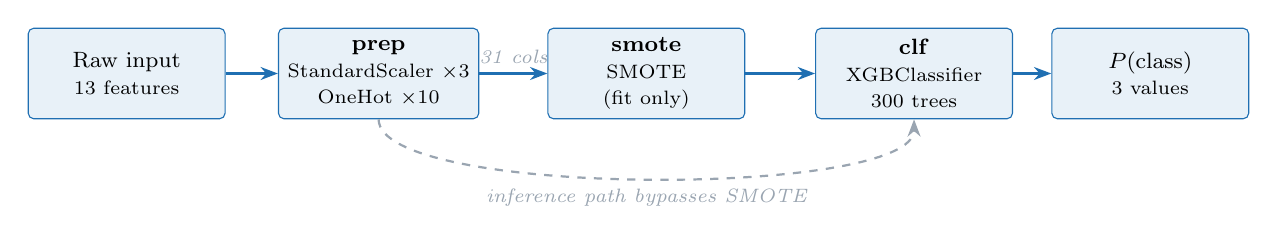
\begin{tikzpicture}[
  font=\footnotesize,
  st/.style={rectangle,rounded corners=2pt,draw=accent,fill=soft,
             minimum width=2.5cm,minimum height=1.15cm,align=center},
  arr/.style={-{Stealth[length=2.2mm]},draw=accent,line width=0.8pt},
  note/.style={font=\scriptsize\itshape,text=grayline,align=center}
]
\node[st] (in)  at (0,0)    {Raw input\\\scriptsize 13 features};
\node[st] (sc)  at (3.2,0)  {\textbf{prep}\\\scriptsize StandardScaler $\times3$\\\scriptsize OneHot $\times10$};
\node[st] (sm)  at (6.6,0)  {\textbf{smote}\\\scriptsize SMOTE\\\scriptsize (fit only)};
\node[st] (xg)  at (10.0,0) {\textbf{clf}\\\scriptsize XGBClassifier\\\scriptsize 300 trees};
\node[st] (out) at (13.0,0) {$P$(class)\\\scriptsize 3 values};

\draw[arr] (in) -- (sc);
\draw[arr] (sc) -- node[note,above]{31 cols} (sm);
\draw[arr] (sm) -- (xg);
\draw[arr] (xg) -- (out);

\draw[arr,dashed,draw=grayline] (sc.south) .. controls +(0,-1.0) and +(0,-1.0) ..
      node[note,below]{inference path bypasses SMOTE} (xg.south);
\end{tikzpicture}
\caption{Training and inference pipeline. The dashed path shows inference, where
the resampling stage is inactive.}
\end{figure}

\subsection{Model Configuration}
\begin{table}[h!]
\centering\small
\begin{tabular}{@{}ll@{\hspace{2.2cm}}ll@{}}
\toprule
\textbf{Parameter} & \textbf{Value} & \textbf{Parameter} & \textbf{Value} \\
\midrule
objective      & multi:softprob & n\_estimators   & 300 \\
num classes    & 3              & max\_depth      & 6 \\
eval\_metric   & mlogloss       & learning\_rate  & 0.1 \\
random\_state  & 42             & encoded classes & High, Low, Medium \\
\bottomrule
\end{tabular}
\caption{XGBoost configuration as recovered from the serialised artefact.}
\end{table}

Note that the label encoder orders classes alphabetically as
(High, Low, Medium), so ``High'' occupies index~0. The implementation therefore
resolves the target class index \emph{by name} rather than by a hard-coded
integer --- a small detail, but one that would otherwise silently generate
explanations for the wrong class.

%=============================================================================
\section{Implementation}

\subsection{Backend}
The service is implemented in Python 3.12 using FastAPI, in 355 lines. It
exposes four endpoints (Table~3). Input validation is declarative: categorical
fields are Python \texttt{str} enumerations and numeric fields carry range
constraints, so FastAPI rejects any out-of-vocabulary or out-of-range value with
HTTP~422 before the model is invoked.

\begin{table}[h!]
\centering\small
\begin{tabular}{@{}llp{7.4cm}@{}}
\toprule
\textbf{Method} & \textbf{Path} & \textbf{Purpose} \\
\midrule
GET  & /health             & Liveness check; returns the model's class labels. \\
GET  & /feature-importance & Global gain-based importance, aggregated to the 13
                             original features. \\
POST & /predict            & Returns predicted class, confidence, and the full
                             probability distribution. \\
POST & /explain            & Returns per-feature SHAP contributions and the
                             ordered recommendation list. \\
\bottomrule
\end{tabular}
\caption{REST API surface.}
\end{table}

\subsection{Frontend}
The client is a React~19 single-page application built with Vite, comprising
approximately 1{,}900 lines across five routes (Home, Risk Test, Knowledge Hub,
Article, FAQ). All styling is hand-written CSS; no UI framework or charting
library is used, which keeps the dependency surface minimal and the production
bundle small.

The risk test itself is a wizard presenting one question at a time, driven by a
four-phase state machine (Figure~3). Questions are defined declaratively in a
single data file, so the questionnaire can be modified without touching
component logic. Choice and yes/no questions auto-advance after a short delay;
slider questions require explicit confirmation, since auto-advancing during a
drag would be incorrect.

\begin{figure}[h!]
\centering
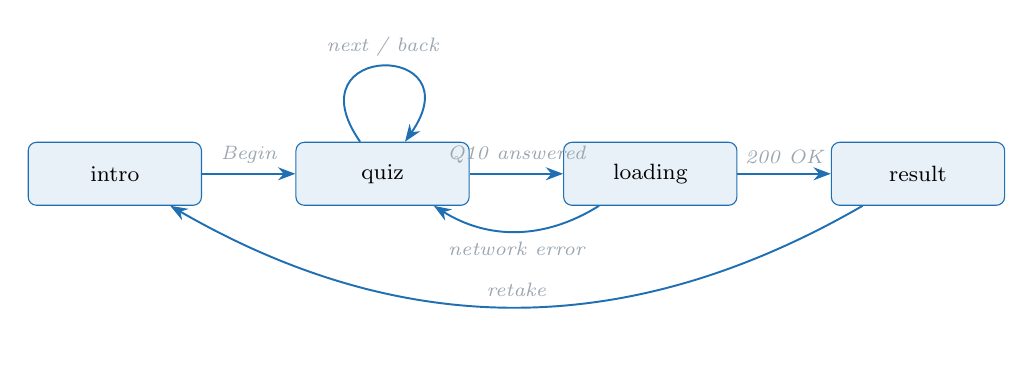
\begin{tikzpicture}[
  font=\footnotesize,
  ph/.style={rectangle,rounded corners=3pt,draw=accent,fill=soft,
             minimum width=2.2cm,minimum height=0.8cm,align=center},
  arr/.style={-{Stealth[length=2.2mm]},draw=accent,line width=0.7pt},
  lbl/.style={font=\scriptsize\itshape,text=grayline}
]
\node[ph] (i) at (0,0)    {intro};
\node[ph] (q) at (3.4,0)  {quiz};
\node[ph] (l) at (6.8,0)  {loading};
\node[ph] (r) at (10.2,0) {result};

\draw[arr] (i) -- node[lbl,above]{Begin} (q);
\draw[arr] (q) -- node[lbl,above]{Q10 answered} (l);
\draw[arr] (l) -- node[lbl,above]{200 OK} (r);
\draw[arr] (q) to[out=125,in=55,looseness=7] node[lbl,above]{next / back} (q);
\draw[arr] (l) to[bend left=32] node[lbl,below]{network error} (q);
\draw[arr] (r) to[bend left=30] node[lbl,above]{retake} (i);
\end{tikzpicture}
\caption{Front-end wizard state machine. A failed request returns the user to
the quiz with their answers preserved.}
\end{figure}

\subsection{The What-If Simulator}
The simulator is the system's most distinctive component. On the result screen
it exposes only the five \emph{modifiable} factors --- physical activity, food
habit, smoking, blood pressure, and BMI --- deliberately excluding age, gender,
and family history, which cannot be acted upon and whose inclusion would be
demoralising rather than useful.

Each adjustment triggers a re-prediction, debounced at 250\,ms to avoid
saturating the API during a slider drag. The result is compared against the
user's baseline on an ordinal rank and reported as a directional change, for
example \textit{``Improved from High $\rightarrow$ Medium''}. This converts the
model from a verdict-generator into an instrument the user can interrogate.

%=============================================================================
\section{Explainability and Recommendations}

\subsection{SHAP Attribution}
A \texttt{TreeExplainer} is constructed once over the trained classifier. For
each request, the input is transformed, SHAP values are computed across the 31
encoded columns, the column corresponding to the High-risk class is selected,
and the values are summed back onto the 13 original features. This aggregation
is mathematically sound because SHAP values are additive in log-odds space.

Figure~4 shows a real explanation produced by the running system for a
52-year-old female, BMI~27.0, high physical activity, never-smoker, healthy
diet, elevated blood pressure, with a family history of diabetes. The system
returned \textbf{Medium} risk.

\begin{figure}[h!]
\centering
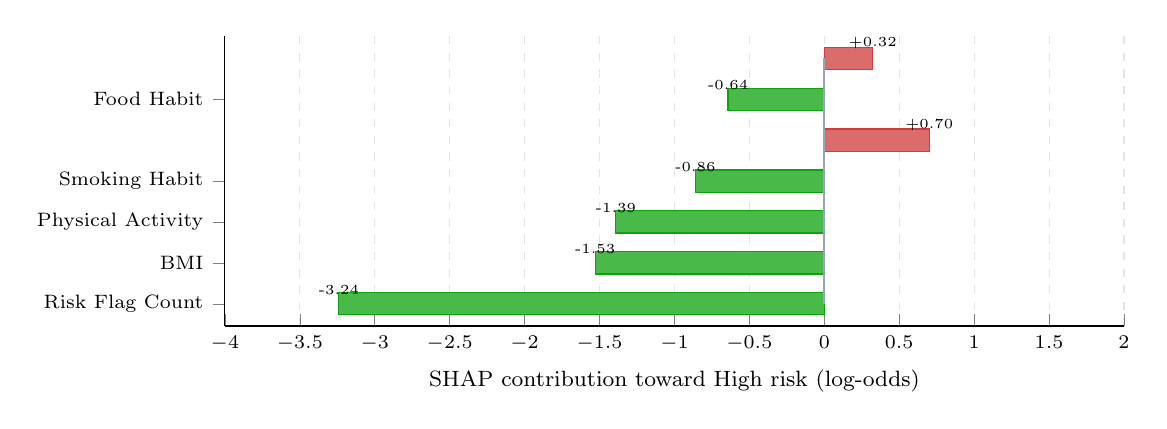
\begin{tikzpicture}
\begin{axis}[
  width=13cm, height=5.4cm,
  xbar, y=0.52cm,
  bar width=8pt,
  xmin=-4, xmax=2,
  xlabel={\footnotesize SHAP contribution toward High risk (log-odds)},
  symbolic y coords={Family History,Food Habit,Age,Smoking Habit,
                     Physical Activity,BMI,Risk Flag Count},
  ytick=data,
  y dir=reverse,
  tick label style={font=\scriptsize},
  label style={font=\scriptsize},
  xmajorgrids, grid style={grayline!30,dashed},
  axis lines*=left,
  enlarge y limits=0.09,
  nodes near coords,
  nodes near coords style={font=\tiny},
  point meta=explicit symbolic
]
\addplot[fill=ok!75,draw=ok,bar shift=0pt] coordinates {
  (-3.2401,Risk Flag Count) [-3.24]
  (-1.5294,BMI) [-1.53]
  (-1.3908,Physical Activity) [-1.39]
  (-0.8603,Smoking Habit) [-0.86]
  (-0.6426,Food Habit) [-0.64]
};
\addplot[fill=bad!75,draw=bad,bar shift=0pt] coordinates {
  (0.7006,Age) [+0.70]
  (0.3232,Family History) [+0.32]
};
\draw[grayline,line width=0.6pt] (axis cs:0,Family History) -- (axis cs:0,Risk Flag Count);
\end{axis}
\end{tikzpicture}
\caption{Actual SHAP output from the deployed system. Green bars (left) lower
predicted risk; red bars (right) raise it. Here the user's healthy diet,
activity level, and absence of smoking pull risk down, while age and family
history push it up.}
\end{figure}

\subsection{Recommendation Engine}
Recommendations are generated by a transparent, hand-authored rule set of eight
clinical guidance rules, each triggered by a threshold on one input. The rules
are deliberately \emph{not} machine-learned: health guidance must be auditable,
and a rule set can be reviewed by a clinician in a way that a generative model
cannot.

The novel element is the ordering. Rather than presenting a fixed list, the
engine sorts triggered recommendations by the SHAP contribution of the feature
that triggered each one, so the advice most relevant to \emph{that particular
user's} risk appears first.

%=============================================================================
\section{Results and Verification}\label{sec:results}

\subsection{Functional Verification}
All endpoints were exercised against a running instance. Results are summarised
in Table~4; all functional tests passed.

\begin{table}[h!]
\centering\small
\begin{tabular}{@{}lll@{}}
\toprule
\textbf{Test} & \textbf{Expected} & \textbf{Observed} \\
\midrule
Artefact loading                & both artefacts load  & pass \\
GET /health                     & classes returned     & \texttt{[High, Low, Medium]} \\
High-risk profile               & High                 & High \\
Low-risk profile                & Low                  & Low \\
Boundary input (age 120, BMI 70)& 200 OK, no NaN bins  & 200 OK \\
Invalid category value          & HTTP 422             & HTTP 422 \\
Out-of-range numeric            & HTTP 422             & HTTP 422 \\
Front-end lint                  & 0 issues             & 0 issues \\
\bottomrule
\end{tabular}
\caption{Functional verification results.}
\end{table}

\subsection{Latency}
Measured on localhost with warmed artefacts: \texttt{/predict} returns in
\textbf{7.2\,ms} and \texttt{/explain} in \textbf{13.2\,ms}. The SHAP
computation therefore costs roughly 6\,ms, which is comfortably fast enough to
drive the what-if simulator interactively.

\subsection{Global Feature Importance}
Figure~5 shows gain-based importance aggregated back to the original features,
as returned by the \texttt{/feature-importance} endpoint.

\begin{figure}[h!]
\centering
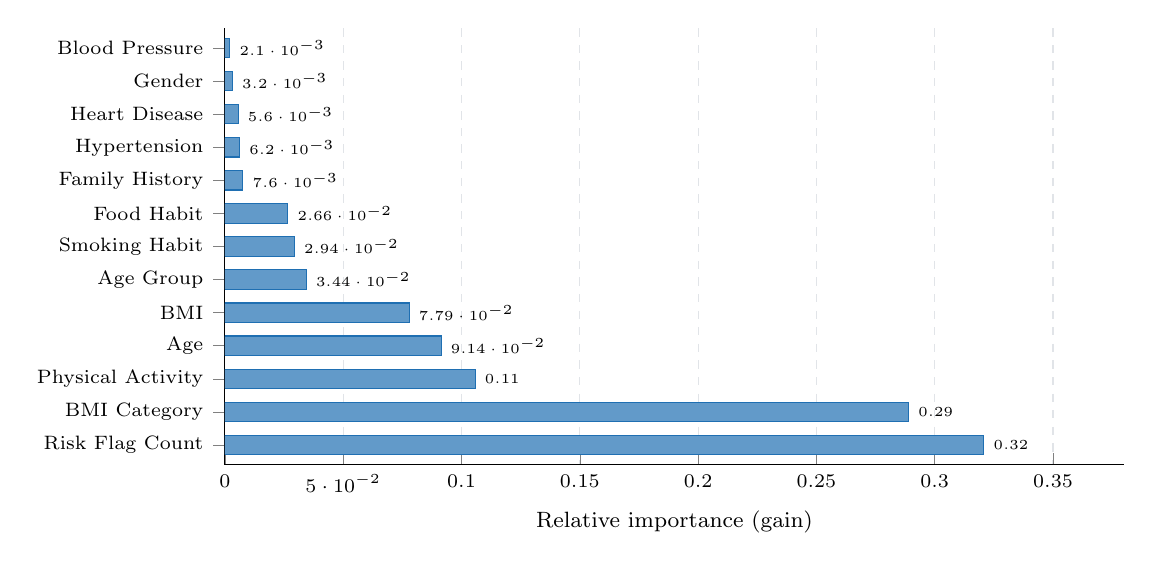
\begin{tikzpicture}
\begin{axis}[
  width=13cm, height=6.2cm,
  xbar, y=0.42cm,
  bar width=7pt,
  xmin=0, xmax=0.38,
  xlabel={\footnotesize Relative importance (gain)},
  symbolic y coords={Blood Pressure,Gender,Heart Disease,Hypertension,
                     Family History,Food Habit,Smoking Habit,Age Group,
                     BMI,Age,Physical Activity,BMI Category,Risk Flag Count},
  ytick=data, y dir=reverse,
  tick label style={font=\scriptsize},
  label style={font=\scriptsize},
  xmajorgrids, grid style={grayline!30,dashed},
  axis lines*=left,
  enlarge y limits=0.05,
  nodes near coords, nodes near coords style={font=\tiny}
]
\addplot[fill=accent!70,draw=accent] coordinates {
  (0.3208,Risk Flag Count) (0.2890,BMI Category) (0.1058,Physical Activity)
  (0.0914,Age) (0.0779,BMI) (0.0344,Age Group) (0.0294,Smoking Habit)
  (0.0266,Food Habit) (0.0076,Family History) (0.0062,Hypertension)
  (0.0056,Heart Disease) (0.0032,Gender) (0.0021,Blood Pressure)
};
\end{axis}
\end{tikzpicture}
\caption{Global feature importance from the deployed model. The engineered
composite \texttt{risk\_flag\_count} dominates; its four constituent inputs
receive correspondingly little individual credit. This concentration effect is
discussed in Section~\ref{sec:remaining}.}
\end{figure}

%=============================================================================
\section{Project Status}

We assess the project at approximately \textbf{80\% completion}. Figure~6 breaks
this down by module.

\begin{figure}[h!]
\centering
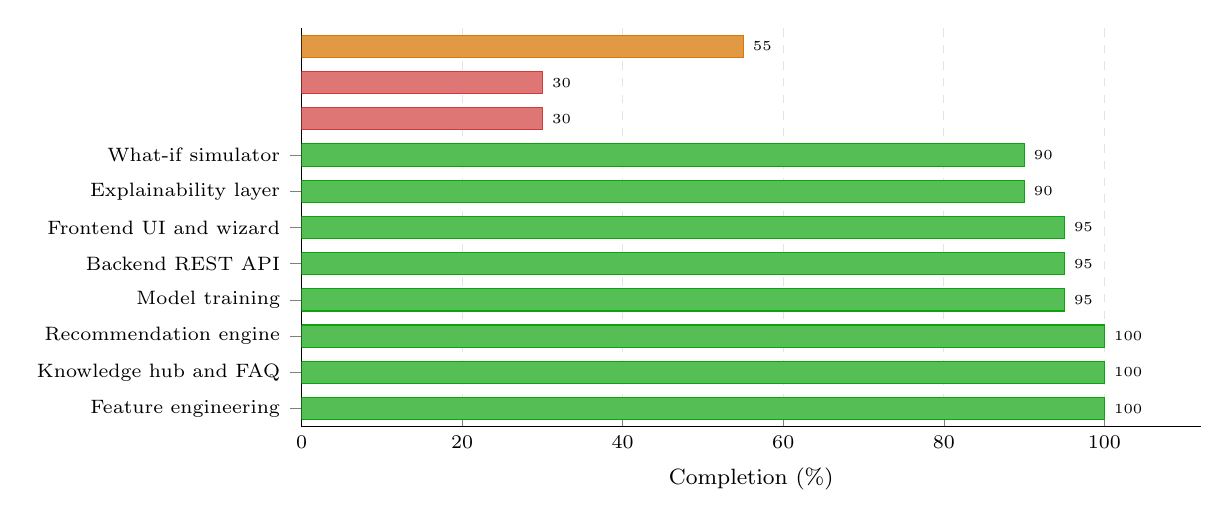
\begin{tikzpicture}
\begin{axis}[
  width=13cm, height=6.4cm,
  xbar, y=0.46cm,
  bar width=8pt,
  xmin=0, xmax=112,
  xtick={0,20,40,60,80,100},
  xlabel={\footnotesize Completion (\%)},
  symbolic y coords={Thesis documentation,Deployment configuration,
                     Testing and validation,What-if simulator,
                     Explainability layer,Frontend UI and wizard,
                     Backend REST API,Model training,
                     Recommendation engine,Knowledge hub and FAQ,
                     Feature engineering},
  ytick=data, y dir=reverse,
  tick label style={font=\scriptsize},
  label style={font=\scriptsize},
  xmajorgrids, grid style={grayline!30,dashed},
  axis lines*=left,
  enlarge y limits=0.05,
  nodes near coords, nodes near coords style={font=\tiny}
]
\addplot[fill=ok!70,draw=ok,bar shift=0pt] coordinates {
  (100,Feature engineering) (100,Knowledge hub and FAQ)
  (100,Recommendation engine) (95,Model training) (95,Backend REST API)
  (95,Frontend UI and wizard) (90,Explainability layer) (90,What-if simulator)
};
\addplot[fill=warn!75,draw=warn,bar shift=0pt] coordinates {
  (55,Thesis documentation)
};
\addplot[fill=bad!70,draw=bad,bar shift=0pt] coordinates {
  (30,Testing and validation) (30,Deployment configuration)
};
\end{axis}
\end{tikzpicture}
\caption{Module-level completion. Unweighted mean across the eleven modules is
80.0\%. Green: complete or near-complete; amber: in progress; red: scheduled.}
\end{figure}

\subsection{Completed}
The entire functional system is built and operational. A user can complete the
questionnaire, receive a risk verdict with a probability breakdown, view a SHAP
explanation, explore counterfactuals interactively, read ordered
recommendations, and browse the knowledge base --- all working end to end.

\subsection{In Progress and Outstanding}
Three areas account for the remaining 20\%: independent model validation, an
automated test suite, and deployment configuration. These are detailed next.

%=============================================================================
\section{Remaining Work and Known Limitations}\label{sec:remaining}

\subsection{Model Validation (Priority 1)}
During verification we observed that the model returns extremely high
confidence across the input space --- in a systematic sweep of 1{,}152 input
combinations, 96\% of predictions carried confidence above 0.99. Further
probing indicated that the predicted class is closely approximated by a simple
additive count of adverse factors.

This pattern is characteristic of a training set whose labels were derived from
the input features rather than from observed clinical outcomes. If so, reported
accuracy would reflect the model successfully recovering a generating rule, not
genuine clinical predictive skill. We regard resolving this as the single most
important remaining task. The planned response is:

\begin{enumerate}[label=\arabic*.]
  \item Audit the provenance of the training data and determine how the labels
        were assigned.
  \item Retrain and validate against a real-world dataset with observed
        outcomes (the UCI Early Stage Diabetes dataset~\cite{islam2020} and the
        CDC BRFSS diabetes indicators are the candidates).
  \item Report a full evaluation --- confusion matrix, per-class
        precision/recall, cross-validated variance --- benchmarked against a
        logistic-regression and a majority-class baseline. The absence of such
        a baseline comparison is what allows an inflated accuracy figure to go
        unchallenged.
\end{enumerate}

We note that the system architecture, API, explanation layer, and interface are
all independent of this issue and will not require rework: only the serialised
model artefact changes.

\subsection{Attribution Concentration}
As Figure~5 shows, the engineered \texttt{risk\_flag\_count} feature absorbs the
attribution belonging to its four constituent inputs, so family history,
hypertension, heart disease, and blood pressure are under-represented in user-
facing explanations. Because \texttt{risk\_flag\_count} is a linear combination
of features the model already receives, we plan to remove it and retrain,
expecting negligible accuracy cost and materially more honest explanations.

\subsection{Testing}
No automated test suite currently exists. The planned suite covers: bin-boundary
correctness in feature engineering, endpoint response schemas, rejection of
invalid input, alignment between probability keys and encoder classes, and
golden-file tests pinning predictions for fixed profiles so that retraining
cannot silently change behaviour.

\subsection{Deployment}
The API base URL is currently hard-coded to localhost, so the built application
cannot yet be hosted. This will move to an environment variable. Production
deployment additionally requires restricting CORS to the front-end origin,
adding rate limiting to the SHAP endpoint, and serving over HTTPS.

\subsection{Accessibility}
The explanation chart encodes direction by colour alone, using precisely the
red/green pairing most affected by common colour vision deficiency. A
non-colour cue and ARIA labelling for the progress bar, choice groups, and
accordion are scheduled.

%=============================================================================
\section{Conclusion}

This project has produced a complete, working, explainable web system for
early-stage diabetes risk screening. Its central argument --- that a risk score
becomes useful only when the user can see why it was assigned and what would
change it --- is realised concretely through a SHAP explanation layer and an
interactive counterfactual simulator, both operating live against the deployed
model at interactive latency.

At approximately 80\% completion, the engineering is substantially finished and
verified. The remaining work is concentrated in validation rather than
construction: establishing that the model's accuracy reflects genuine predictive
skill, backing that claim with a rigorous evaluation against real clinical data
and appropriate baselines, and hardening the system for deployment. We consider
identifying the validation concern at this stage --- rather than at submission
--- to be a substantive result of the verification effort, and the remaining
schedule is built around resolving it.

%=============================================================================
\begin{thebibliography}{9}
\small
\bibitem{idf2021} International Diabetes Federation.
  \textit{IDF Diabetes Atlas}, 10th ed. Brussels, Belgium, 2021.
\bibitem{dpp2002} W.~C. Knowler et al. ``Reduction in the incidence of type~2
  diabetes with lifestyle intervention or metformin.''
  \textit{New England Journal of Medicine}, 346(6):393--403, 2002.
\bibitem{xgboost} T.~Chen and C.~Guestrin. ``XGBoost: A scalable tree boosting
  system.'' In \textit{Proc. 22nd ACM SIGKDD}, pp.~785--794, 2016.
\bibitem{shap} S.~M. Lundberg and S.-I. Lee. ``A unified approach to
  interpreting model predictions.'' In \textit{Advances in Neural Information
  Processing Systems 30}, pp.~4765--4774, 2017.
\bibitem{treeshap} S.~M. Lundberg et al. ``From local explanations to global
  understanding with explainable AI for trees.'' \textit{Nature Machine
  Intelligence}, 2(1):56--67, 2020.
\bibitem{smote} N.~V. Chawla et al. ``SMOTE: Synthetic minority over-sampling
  technique.'' \textit{Journal of Artificial Intelligence Research},
  16:321--357, 2002.
\bibitem{islam2020} M.~M.~F. Islam et al. ``Likelihood prediction of diabetes at
  early stage using data mining techniques.'' In \textit{Computer Vision and
  Machine Intelligence in Medical Image Analysis}, Springer, pp.~113--125, 2020.
\bibitem{sklearn} F.~Pedregosa et al. ``Scikit-learn: Machine learning in
  Python.'' \textit{Journal of Machine Learning Research}, 12:2825--2830, 2011.
\bibitem{imblearn} G.~Lema{\^i}tre, F.~Nogueira, and C.~K. Aridas.
  ``Imbalanced-learn: A Python toolbox to tackle the curse of imbalanced
  datasets.'' \textit{Journal of Machine Learning Research}, 18(17):1--5, 2017.
\end{thebibliography}

\end{document}
